V následující kapitole si popíšeme něco málo o sestavě, která byla pro účely testování a srovnáváni výkonu virtualizačních nástrojů použita. Krom hardwarové výbavy testovacího stroje, což je základní minimum, které by mělo být uvedeno v každé práci zabývající se testováním výkonu určitých softwarových produktů, si také uvedeme operační systém a jeho přesnou verzi. Pro zvýšení vypovídající hodnoty následujících testů, zde uvedu i přesné verze jednotlivých nástrojů použitých při testování.

\section{Testovací sestava}
\subsection{Základní deska}
Základem celého počítače je deska 880GMH/U3S3 od firmy ASRock. Důvodem pro její zvolení byla údajná podpora nejnovější rodiny AMD procesorů Bulldozer a také její podpora taktování. Během osazení této desky jednim z nových procesorů, se ukázalo, že podporu bulldozerů sice deska má. Bohužel až s nejnovější verzí BIOSu. Tu samozřejmě většina prodávaných kusů neměla. Bylo tedy nutno použít starší AMD procesor se socketem AM2+ a vyšší. A následně provést update BIOSu. Poté už vše fungovalo v pořádku.
\subsubsection{Přehled kompletních parametrů}
\begin{itemize}
  \item Podpora pro AM3+ procesory, až 8 jader
  \item 100\,\% pevných kondenzátorů (delší životnost) 
  \item Podpora pro Dual Channel DDR3 2000(OC)
  \item Podpora ATI™ Hybrid CrossFireX™
  \item Integrovaná GPU AMD Radeon HD 4250 graphics, DX10.1 class iGPU, Shader Model 4.1
  \item Video výstupy : D-Sub, DVI-D a HDMI
  \item 2 x USB 3.0, 2 x SATA3, C.C.R. (Combo Cooler Retention Module)
  \item Podpora dalších technologií: AXTU, Graphical UEFI, Instant Boot, Instant Flash, APP Charger, SmartView
\end{itemize}

\subsection{Procesor}
Jak už jsme se výše zmínil, použit byl procesor od firmy AMD se socketem AM3+ . Jednalo se o jeden z prvních modelů nové rodiny Bulldozer. Přesné označení procesoru je AMD FX-4100. Jedná se o procesor se čtyřmi jádry, kde každý z nich je v základním nastavení taktován na frekvenci 3,6 GHz (respektive 3,7 -- 3,8 v Turbo módu). Díky odemknutému násobiči je tento procesor přímo předurčen pro přetaktování. V době testů byl však ponechán na jeho základních frekvencí s vypnutým turbo boostem.

\subsubsection{Podrobné parametry}
\begin{itemize}
  \item Socket: AM3+
  \item L2 cache: 4 MB
  \item Frekvence: 3600 MHz
  \item Typ: AMD FX
  \item Model: FX-4100
  \item Počet jader: 4
  \item Operační módy: 32-bit a 64-bit
  \item L3 cache: 8 MB
  \item Výrobní proces: 32\,nm
  \item TDP: 95\,W
\end{itemize}

\subsection{Disky}
Počítačová sestava je vybavena dvěma pevnými disky jedním rychlým systémovým SSD diskem Verbatim o kapacitě 128\,GB, a druhým datovým SATA-II diskem Samsung o kapacitě 1\,GB.
\subsubsection{Parametry systémového disku}
\begin{itemize}
  \item Výrobce: Verbatim
  \item Model: SSD Black Edition
  \item Kapacita: 128\,GB
  \item Rozhraní: Serial ATA II
  \item Průměrný vyhledávací čas: 0.1\,ms
  \item Rychlost čtení: 270\,MB/s
  \item Rychlost zápisu: 225\,MB/s
  \item Rychlost přenosu dat: 3\,Gbit/s
  \item Speciální funkce: podpora TRIM a NCQ
\end{itemize}

\subsubsection{Parametry datového disku}
\begin{itemize}
  \item Výrobce: Samsung
  \item Model: SpinPoint F1
  \item Kapacita: 1000\,GB 
  \item Průměrný vyhledávací čas: 8.9\,ms  
  \item Rychlost otáčení ploten: 7200\,rpm
  \item Vyrovnávací paměť: 32\,MB
  \item Rozhraní: Serial ATA II
  \item Rychlost přenosu dat: 3\,Gbit/s
  \item Speciální funkce: NCQ
\end{itemize}

\subsection{Operační paměť}
Celkově počítač obsahuje čtyři paměťové moduly, kde každý má velikost 4\,GB a jsou spárovány po dvou, tak aby bylo využito podpory dual-channel. Dohromady tedy sestava disponuje 16\,GB RAM. Což je pro testovací účely víc než dostačující.
\section{Operační systém}
\subsection{Zvolená platforma}
První věcí, kterou bylo třeba při výběru OS rozhodnou byla platforma potažmo jádro operačního systému. Jelikož několik zvolených virtualizačních nástrojů podporuje pouze Linux. Nebyl důvod se moc rozmýšlet. Chvíli jsem uvažoval o některé variantě BSD systému, jelikož by zde šla teoreticky rozchodit většina zvolených nástrojů, a ty které by zde nešli, mají svoji alternativu. Ale nakonec jsem tuto myšlenku potlačil, jelikož Linux je rozšířenější, a dá se předpokládat, že pokud někdo bude některý ze zmiňovaných virtualizačních nástrojů nasazovat, tak to bude právě na Linuxu.

\subsection{Volba distribuce}
Dalším krokem po vybrání Linuxu jako hlavní platformy, na níž budu provádět veškeré testování, byla volba distribuce. Zde to již bylo o něco složitější, jelikož existuje skoro bezpočet distribucí, kde každá má své klady a zápory. Prvním rozhodnutím, které zúžilo možný počet kandidátů, byla snaha vybrat distribuci, poskytující dostatek dokumentace, popisující zprovoznění pokud možno co největšího počtu z vybraných virtualizačních nástrojů. Druhým kritériem byla co největší aktuálnost dostupných verzí jednotlivých softwarových komponent distribuce.

Důvodem proč jsem hledal distribuci s co nejnovějšími verzemi aplikací, byl fakt, že virtualizační nástroje se velmi rychle vyvíjí a já chci poskytnout co nejvěrohodnější výsledky těchto nástrojů v dnešní době. Což by mělo mít za výhodu aktuálnost mých výsledků i po delší době. Tento přístup má i své stinné stránky. Nejnovější verze sebou krom nejnovějších vylepšení mohou nést i některé nové chyby, což může vést k určitým nestabilitám dané aplikace. Jelikož většina použitého software bude ve stabilních verzích, není toto riziko příliš vysoké.

Oba dva předchozí požadavky nejlépe splňovaly dvě distribuce. Jednou z nich bylo Ubuntu, které patří mezi jednu z nejrozšířenějších distribucí Linuxu. Tudíž pro ni existuje i spousta předpřipravených balíčků z potřebnými aplikacemi a nástroji. A také kolem ní existuje velká komunita, kam se může člověk obrátit s případnými problémy. Druhým adeptem byla o něco méně rozšířená, avšak v poslední době velmi populární distribuce s názvem Arch Linux. Jeho hlavní výhodou jsou opravdu velmi aktuální verze programů a aplikací. Jedná se o tzv. rolling updates distribuci, to znamená, že se nevydávají jednotlivé verze distribuce, ale distribuce je aktualizovaná postupně pomocí aktualizací, kde tyto aktualizace nejsou pouze opravné verze, ale i zcela nové verze jednotlivých komponent. Co se komunity týče, tak ačkoliv není tak rozsáhlá jako u předchozího adepta, tak díky své aktivitě a odborným znalostem lidí pohybující se okolo této distribuce, svojí kvalitou komunitu okolo Ubuntu předčí. Další věcí, která mi při rozhodování mezi těmito dvěma adepty pomohla rozhodnout, byla podpora vytváření vlastních balíčků. Žádná jiná mně známá distribuce nenabízí tak jednoduchý způsob tvorby balíčků s vlastním software, jako má Arch Linux.

Nakonec jsem se tedy rozhodl pro Arch Linux. Jeho instalaci zde probírat nebudu, jelikož je to mimo rozsah této práce. Případné zájemce odkáži na wiki stránku zabývající se instalací této distribuce, která je dostupná hned v několika jazykových mutací\footnote{\url{https://wiki.archlinux.org/index.php/Official\_Installation\_Guide}}
\footnote{\url{https://wiki.archlinux.org/index.php/Official\_Installation\_Guide\_(Česky)}}
\footnote{\url{https://wiki.archlinux.org/index.php/Official\_Installation\_Guide\_(Slovenský)}}.

\subsection{Virtualizované systémy a jejich konfigurace}
Jak už jsem psal v této kapitole jako operační systém pro hostitele jsem si zvolil Arch Linux. V případě hosta jsem se rozhodl hned pro dvě distribuce. Důvodem bylo zjistit, zda rozdílné distribuce běží ve virtualizovaném prostředí odlišně. Jedním vybraným kandidátem je opět Arch Linux a jako další byla zvolena Fedora Core 16. Důvodem výběru těchto dvou kandidátů je především jejich aktuálnost, hlavně jejich aktuální verze jádra. Což by mělo mít za následek, co možná nejpokročilejší podporu aktuálních verzí virtualizačních nástrojů, a také zaručovat co možná největší kompatibilitu s jádrem hostitele. U Fedory jsem vzlal taky v potaz, že je vývojovou verzí pro komerční RedHat Linux.

Obě tyto distribuce byli ponechány během testování v základním nastavení. Tím mám namysli, že zde nebyli prováděny žádné zásahy, které by ovlivňovali jejich výkonnost v testech (změna konfigurace jádra a podobně). Samozřejmě po dobu testování nebyly na těchto systémech prováděny aktualizace, tak aby všechny výsledky byly co nejvěrohodnější. Jediné úpravy byly ty, které přímo souviseli s podporou dané virtualizační technologie, jako například doinstalování rozšíření pro VirtualBox atd.

U obou dvou distribucí i u všech virtualizačních technologií jsem se snažil vytvořit pokud možno co nejhomogennější prostředí. Všem virtuálním systémům bylo vždy přiděleno jen jedno jádro a 2048\,MB operační paměti.

Krom těchto dvou hostů s operačním systémem Linux, jsem zvolil i jednoho zástupce s operačním systémem Microsoft Windows. Jelikož kontejnerová řešení jako je LXC, Linux-VServer a OpenVZ podporují jen Linuxové hosty. Bude Windows host testován pouze v KVM, VirtualBox a Xen hypervizoru.

\section{Příprava virtualizačních nástrojů}
V této sekci si lehce popíšeme instalaci a konfiguraci testovaných nástrojů a dalších podpůrných utilit. Rád bych upozornil, že následující text předpokládá pokročilou znalost administrace OS Linux a alespoň částečnou znalost distribuce Arch Linux.
\subsection{Instalace}
\subsubsection{\xen}
Xen hypervizor není dostupný v oficiálních repositářích Arch Linuxu, ale za pomocí ABS (\emph{\textbf{A}rch \textbf{B}uild \textbf{S}ystem}) jsem si sestavit vlastní balíček. K tomuto účelu byl použit PKGBUILD, který je součástí přílohy této práce viz. \ref{xenpkgbuild}.

Po vytvoření a instalaci Xen hypervizoru je ještě třeba správně nastavit zavaděč např. GRUB, tak aby bylo možné najet do systému s podporou Xen hypervizoru. Já jsem využil existující (součást vytvořeného instalačního balíčku) šablony pro GRUB2, která mi při generování konfiguračního souboru pro zavaděč automaticky rozpoznala a nastavila příslušnou sekci pro Xen hypervizor.
\newpage
Pokud je xen správně nainstalován a zavaděč správně nastaven. Mělo by jít po restartu najet do systému s podporou xen. V mém případě se však ukázalo, že aktuální verze jádra 3.3 obsahuje chybu, která neumožňuje běh Xen hypervizoru. Tento problém je vyřešen workaroundem ve vývojové verzi jádra 3.4 a plně vyřešen bude až ve verzi 3.5. Já abych mohl pokračovat jsem využil patch, který byl použit právě pro nadcházející jádro 3.4 \footnote{\url{http://git.kernel.org/?p=linux/kernel/git/torvalds/linux.git;a=commitdiff;h=2531d64b6fe2724dc432b67d8dc66bd45621da0b;hp=e95ae5a4939c52ccab02a49238d5d15d492b2598}}.

Po aplikaci tohoto workaraoundu na distribuční jádro, jsem byl po restartu systému již schopný nabootovat do Dom0 hosta běžícím na Xen hypervizoru.

\subsubsection{KVM}
Instalace a zprovoznění KVM byla spolu s VirtualBoxem asi jedna z nejsnazších a nejméně problematických. Jelikož samotný KVM "`hypervizor"' je součástí jádra, stačilo doinstalovat jen nástroje pro práci s ním. Pro práci s KVM se využívá upravená verze emulačního software Qemu. Ta se v repositáři nachází pod názvem \texttt{qemu-kvm}.

Já jsme nakonec nepoužil přímo verzi z oficiálních repositářů, jelikož neobsahovala podporu pro SPICE protokol. SPICE protokol je celkem nová záležitost, která přináší pro KVM hosty podporu integrace kurzoru myši a další vylepšení známá v konkurenčních nástrojích. Jedinou změnou co bylo potřeba udělat pro zapnutí podpory SPICE, bylo přidat do konfigurace sestavení volbu \texttt{---enable-spice}. A ještě před sestavením takto upravené verze \texttt{qemu-kvm}, doinstalovat balíček \texttt{spice-protocol}.

Pokud chceme využívat KVM jako obyčejný uživatel, musíme jeho účet přidat do skupiny \texttt{kvm}.

\subsubsection{UML}
User Mode Linux se skládá z dvou částí. První část \texttt{uml\_utilities} je dostupná v komunitním repositáři a jedná se o podpůrné nástroje využívané nejen pro samotné UML. Druhou částí samotné UML, jedná se vlastně o speciální verzi jádra Linuxu, která je spustitelná jako normální aplikace.

 Ta je dostupná jen jako PKGBUILD v AURu (\textit{\textbf{A}rch \textbf{U}ser \textbf{R}epository}). K instalaci balíčků z AURu je možné použít různé utility. Já použil například nástroj zvaný \texttt{yaourt}. Což je tuším zkratka ze slov Yet Another User Repository Tool.
\subsubsection{VirtualBox}
Jak už jsem se zmínil instalace VirtualBoxu je celkem bezproblémová. Jelikož je VirtualBox velmi populární a dobře podporovaný. Jediné co je třeba udělat, je nainstalovat si balíčky \texttt{virtualbox} a \texttt{virtualbox-modules}. Případně ještě balíček \texttt{virtualbox-additions}, který obsahuje různá rozšíření pro hosty (integrace kurzoru myši, ovladače pro akceleraci grafiky\dots).

Tak jak u KVM je třeba se přidat do skupiny \texttt{kvm}, tak pro používaní VirtualBoxu obyčejným uživatelem, je třeba jej přidat do skupiny \texttt{vboxusers}. Tato skupina není standardně součástí systému, vytvoří se až po instalaci balíčků VirtualBoxu.
\subsubsection{LXC}
Všechny technologie, které Linux Containers využívá jsou již součástí distribučního jádra. Jediné co je tedy potřeba doinstalovat, jsou utility pro práci s LXC. Ty sice nejsou součástí hlavních repositářů, ale jsou opět dostupné v AURu. Takže opět stačí nechat si vytvořit a nainstalovat balíček. To se provede například tímto příkazem:
\begin{verbatim}
  yaourt -S lxc
\end{verbatim}
\subsubsection{Linux-VServer}
Linux-VServer na rozdíl od LXC využívá svoje vlastní prostředky, které nejsou součástí distribučního jádra Linuxu. Proto je potřeba si toto jádro nejprve opatchovat a rozšířit jej tak, o požadovanou funkcionalitu. Poté si opatchované jádro nakonfigurovat (po zapínat vše potřebné), zkompilovat a nainstalovat. Toto všechno vyžaduje spoustu znalostí a nezkušeným lidem, to může zabrat i celý den. Naštěstí v AURu již existuje předpřipravený PKGBUILD, který to vše udělá za nás.
\\
Takže pro nainstalování Linux-VServeru a podpůrných nástrojů i se závislostmi stačí zadat příkaz:
\begin{verbatim}
  yaourt -S linux-vserver util-vserver 
\end{verbatim}

Pokud vše proběhne v pořádku, měl by být Linux-VServer nainstalován. Jediné co je ještě potřeba je přidat do zavaděče možnost bootovat s jádra s podporou Linux-VServer.
Jelikož mám nainstalovaný zavaděč Grub2 a podpůrnou utility os-prober, stačí zadat příkaz pro vygenerování konfigurace k zavaděči:
\begin{verbatim}
  grub-mkconfig -o /boot/grub/grub.cfg 
\end{verbatim}
\subsubsection{Libvirt}
Libvirt není přímo samostatné virtualizační řešení, a jak název napovídá jedná se o knihovnu. Přesněji řečeno knihovna je jen malá část, libvirt je spíše toolkit umožnující správu několika různých virtualizačních řešení pomocí jednoho rozhraní. Toto je velmi výhodné, protože v ideálním případě se stačí naučit používat jen jeden nástroj pro libovolnou virtualizační technologii. Seznam podporovaných virtualizačních nástrojů naleznete na oficiálních stránkách projektu CitND.

Instalaci libvirt lze uskutečnit instalací s repositářů. Ale jak už je zvykem, opět zde něco chybí. Tím co chybí je podpora pro Xen hypervizor. Ta je v oficiálním balíčku vypnuta. Proto je třeba si opět upravit PKGBUILD a podporu pro požadované vlastnosti si zapnout. Díky ABS to není žádný problém a zabere to jen pár minut.
\subsubsection{Virtual Machine Manager}
Je sice pěkné mít toolkit jako je libvirt, který nám nabízí programátorské rozhraní pro různé virtualizační nástroje. Ale jelikož lidé jsou tvoří líní, a určitě by se jim spíše líbilo grafické rozhraní, kde si vše mohou pěkně a přehledně nastavovat pomocí myši a klávesnice. Tak vznikl projekt Virtual Machine Monitor (zkráceně Virt-manager). Což není nic jiného než ono grafické udělátko nad libvirt. Jak vypadá si můžete prohlédnout na obrázkách \ref{obr:vmm} a \ref{obr:vmmc}

\begin{figure}[h!]
  \centering
  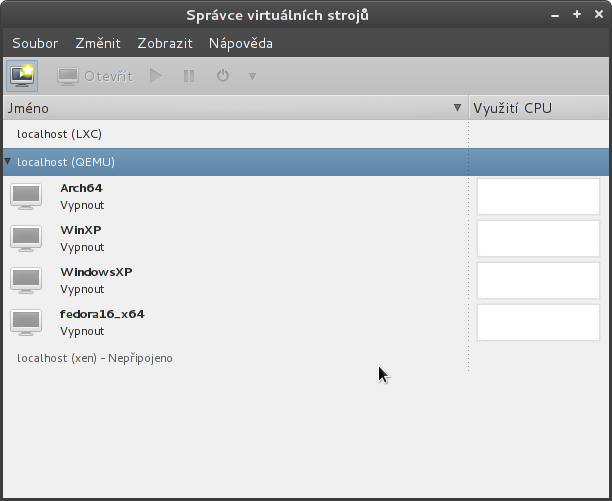
\includegraphics[width=12cm]{obr/vmm}
  \caption{Základní ono Virtual Machine Manageru.}
  \label{obr:vmm}
\end{figure}
\begin{figure}[h!]
  \centering
  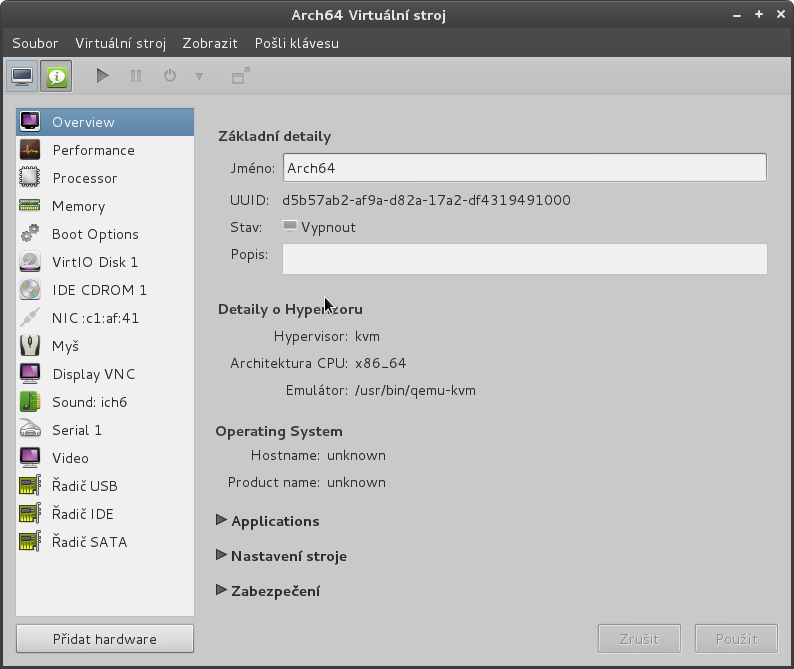
\includegraphics[width=12cm]{obr/vmmc}
  \caption{Okno pro konfiguraci virtuálního stroje.}
  \label{obr:vmmc}
\end{figure}
\newpage
Instalace Virt-manager je snadná, jelikož je součástí komunitního repositáře a není třeba jej nijak upravovat, stačí jej nainstalovat pomocí nástroje pro správu balíčků \texttt{pacman}, případně stejně dobře poslouží i již zmiňovaný \texttt{yaourt}, který je nadstavbou a umí pracovat i s normálními repozitáři.
\subsection{Konfigurace a použití}
\subsubsection{\xen}
Aby bylo možné používat, pro práci s Xen hypervizorem, Virt-manager, je zapotřebí mít nainstalován a spuštěn libvirt démon. Démon je součástí balíčku libvirt a démoni se v Arch Linuxu spouští příkazem \verb!rc.d start !\textit{\texttt{název}\texttt{\_}\texttt{démona}}. V našem případě by jsme tedy spustili příkaz \verb!rc.d start libvirtd!. Krom libvirt démona je potřeba nastartovat i další démony zajišťující běh Xen služeb. Jsou to démoni \texttt{xencommons} a \texttt{xend}. Případně \texttt{xendomains}, který má na starost automatické nastartování nainstalovaných DomU hostů.

Pozor na fakt, že v základním nastavení by nám libvirt neuměl komunikovat s Xen démonem. proto poprvé než spustíme démony, musíme xend nakonfigurovat. Celá konfigurace spočívá v nastavení (odkomentování) jednoho (dvou) řádků v souboru \verb!/etc/xen/xend-config.sxp!. Po úpravě a odstranění komentářů výsledný konfigurační soubor vypadá následovně:
\begin{alltt}
  \textbf{(xend-http-server yes)}
  \textbf{(xend-tcp-xmlrpc-server yes)}
  (xend-relocation-server yes)
  (xend-relocation-hosts-allow '^localhost$ ^localhost\textbackslash\textbackslash.localdomain$')
  (network-script network-bridge)
  (vif-script vif-bridge)
  (dom0-min-mem 196)
  (enable-dom0-ballooning yes)
  (total_available_memory 0) 
  (dom0-cpus 0)
  (vncpasswd '')
\end{alltt}

Tučně jsou zvýrazněny ty řádky, které bylo třeba odkomentovat. Po této změně a nastartování výše zmíněných démony, by již mělo jít použít Virt-manager ke správě DomU hostů.

Samotný postup vytvoření nového virtuálního stroje se pomocí Virt-manageru u jednotlivých virtualizací skoro neliší, takže si jej podrobněji ukážeme později v textu popisujícím konfiguraci KVM. Xen hosti se dají ovládat i pomocí několika dalších nástrojů. Tím úplně základním je příkaz \texttt{xm}, který je přímo součástí xenu. Jeho kompletní seznam možných operací a parametrů si vypíšeme příkazem \texttt{xm help}. Ty nejpoužívanější a nejdůležitější jsou po vypsání nápovědy uvedeny jako první. Jedná se o příkazy pro vytváření a mazání DomU hostů, jejich nastartování a vypnutí atd. Na obrázku \ref{fig:xm} vidíme několik prvních z nich.

Ačkoliv jsem po většinu času využíval kombinaci libvirt a Virt-manager, tak občas se mi stalo, že se mi ve Virt-manageru přestali zobrazovat běžící hosti. Potom bylo potřeba se na ně připojit právě pomocí utility xm. Buď pomocí příkazu \verb!xm console název_hosta! pokud byl host správně nastaven a měl spuštěný terminál, nebo případně pomocí VNC protokolu příkazem \verb!xm vncviewer název_hosta!. Aby bylo možné použít VNC spojení, je třeba mít nainstalovaný balíček \texttt{tightvnc}.
\begin{figure}[h!]
  \centering
\begin{alltt}
    console              Attach to <Domain>'s console.                     
    vncviewer            Attach to <Domain>'s VNC server.                  
    create               Create a domain based on <ConfigFile>.            
    new                  Adds a domain to Xend domain management           
    delete               Remove a domain from Xend domain management.      
    destroy              Terminate a domain immediately.                   
    domid                Convert a domain name to domain id.               
    domname              Convert a domain id to domain name.               
    dump-core            Dump core for a specific domain.                  
    list                 List information about all/some domains.          
    mem-max              Set the maximum amount reservation for a domain.  
    mem-set              Set the current memory usage for a domain.        
    migrate              Migrate a domain to another machine.              
    pause                Pause execution of a domain.                      
    reboot               Reboot a domain.                                  
    rename               Rename a domain.                                  
    reset                Reset a domain.                                   
    restore              Restore a domain from a saved state.              
    resume               Resume a Xend managed domain                      
    save                 Save a domain state to restore later.             
    shutdown             Shutdown a domain.                                
    start                Start a Xend managed domain
    \dots
\end{alltt}
\caption{Výpis několika prvních podpříkazů xm utility.}
  \label{fig:xm}
\end{figure}
\subsubsection{KVM}
U KVM je situace o něco jednoduší, jelikož zde není potřeba nic konfigurovat. Jediné co je potřeba pro správnou funkčnost libvirt a Virt-manager, jsou načtené moduly \texttt{kvm} a \texttt{kvm-amd} nebo \texttt{kvm-intel}. Potom už nám nic nebrání ke spuštění libvirt démona a následného spuštění Virt-manageru, kde si po vytvoření spojení s KVM, můžeme spravovat naše virtuální stroje. Jak to přesně provést to si teď popíšeme a ukážeme na několika obrázkách.
\begin{figure}[h!]
  \centering
  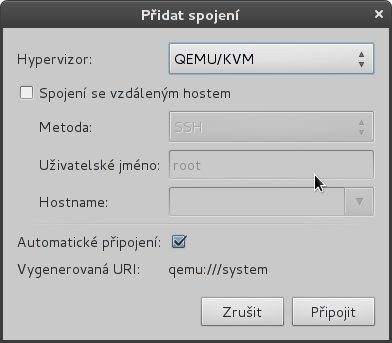
\includegraphics[width=12cm]{obr/vmmconnection}
  \caption{Okno pro nastavení spojení s hypervizorem.}
  \label{obr:vmmconnection}
\end{figure}

Po spuštění Virt-manageru se nám zobrazí hlavní okno (obrázek \ref{obr:vmm}). V tomto okně zvolíme v menu \emph{soubor} položku \emph{Přidat spojení\dots}. Tím se nám zobrazí dialogové okno jako na obrázku \ref{obr:vmmconnection}. Zde si zvolíme typ hypervizoru, který chceme používat (KVM, XEN, LXC\dots). V našem případě to bude varianta QEMU/KVM.

Dále zde můžeme nastavit zda chceme spravovat virtuální stroje bežící na tomto stroji, nebo na některém vzdáleném pomocí SSH protokolu. Jelikož v mém případě se vše testuje na jednom stroji, tak nechám možnost \emph{Spojení se vzdáleným hostem} odškrtnutou. 

Poslední co se zde dá nastavit je možnost automatického připojování v případě zapnutí Virt-manageru. Jelikož testuji několik různých virtualizačních nástrojů a ne všechny mohou běžet současně, je pro mě lepší tuto volbu nechat vypnutou a startovat si spojení na žádost (poklepáním na příslušný záznam spojení v hlavním okně). Pokud je vše správně nastaveno měly by se po spojení načíst existující virtuální stroje (pokud samozřejmě již máme nějaké vytvořené).

Samotná tvorba virtuálních strojů je velmi snadná. Slouží k tomu průvodce, který se spustí první ikonkou v nástrojové liště (ikonka počítače s šipkou a hvězdičkou). Tento průvodce nás postupně provede přidáním nového virtuálního stroje (název, určení typu OS, architektury, odkud instalovat, velikosti disků, paměti a počet použitých CPU jader\dots). Jednotlivými kroky se zde podrobně zabývat nebudu, jelikož je to mimo rozsah této práce.

Tak jako u Xenu i KVM se dá ovládat bez použití Virt-manageru. Jak už jsem psal KVM je silně svázáno s Qemu, takže se dá používat v podstatě úplně stejně. Jen s tím rozdílem že se příkazu \texttt{qemu} předá parametr (v nejnovějších verzích už není pravda, akcelerace je automaticky zapnuta), který zapíná KVM akceleraci. Krom konzolového \texttt{qemu} se dají vcelku snadno použít i různé grafické nadstavby jako je Aqemu nebo Qemu-launcher. Další možností jak KVM ovládat (spíše do budoucna) je utilita linux-kvm \footnote{\url{https://github.com/penberg/linux-kvm}}, která je momentálně ještě ve vývoji a nepodařilo se mi ji pořádně zprovoznit.
\subsubsection{UML}
UML jak jsem již psal je v podstatě jádro zkompilované do tvaru normální binární aplikace. Veškerá konfigurace probíhá stejně jako u normálního jádra pomocí parametrů. S tím rozdílem že zde se jádro nespouští přes zavaděč ale přímo jako aplikace.

K tomu abychom mohli vytvořit virtuální stroj pro UML potřebujeme mít připravený obraz disku se systémem, který chceme virtualizovat. Takový disk se dá pro různé distribuce nalézt již připravený, jelikož má využití i například pro LXC, Linux-VServer nebo klidně i pro KVM a Xen. Druhá možnost je si disk připravit ručně pomocí příkazu \texttt{dd} si naalokovat potřebnou velikost, vytvořit na něm souborový systém a nahrát potřebné systémové soubory. Natažení systému na připravený disk se dá provést buď jednoduchým zkopírováním struktury existujícího systému, nebo pomocí různých nástrojů k tomu určených.

Například pro vytvoření 5\,GB obrazu s operačním systémem Arch Linux by jsme zadali následující sekvenci příkazů:
\begin{verbatim}
  [root@KozziFX kozzi]# dd if=/dev/zero of=arch_rootfs bs=1MB count=5000
  [root@KozziFX kozzi]# mke2fs -F arch_rootfs
  [root@KozziFX kozzi]# mount -o loop arch_rootfs /mnt
  [root@KozziFX kozzi]# mkdir -p /mnt/var/lib/pacman
  [root@KozziFX kozzi]# pacman -Sy base -r /mnt
  [root@KozziFX kozzi]# cd /mnt/dev
  [root@KozziFX kozzi]# mknod --mode=660 ubd0 b 98 0
  [root@KozziFX kozzi]# chown root:disk ubd0
  [root@KozziFX kozzi]# echo "/dev/ubd0 / ext2 defaults 0 0" >> /etc/fstab
  [root@KozziFX kozzi]# umount /mnt
\end{verbatim}
První pětice příkazů vytvoří obraz na který nahraje základní systém Arch Linuxu. Zajímavější jež příkaz \texttt{mknod}, který vytváří blokové zařízení \texttt{ubd0}, které je pak přidáno jako rootfs. Důvodem proč je toto potřeba je, že UML svůj emulovaný disk mapuje právě na toto zařízení, a pokud by virtualizovaný systém neobsahoval toto zařízení, nemohl by se systém nastartovat a skončilo by to hláškou kernel panic.

Dalším krokem je připravení síťové infrastruktury pro hosta, jelikož abychom mohli nějak s virtualizovaným hostem pracovat a komunikovat, určitě budeme potřebovat, aby měl připojení alespoň do naší vnitřní sítě. UML podporuje několik způsobů (typů) připojení do sítě. Asi nejsnazší je využití nástroje \texttt{vde} (Virtual Distributed Ethernet), který se hojně využívá i u dalších podobných nástrojů jako je UML.

Jediné co je potřeba udělat aby v UML hostovi síť fungovala jsou tyto tři příkazy:
\begin{verbatim}
  [root@KozziFX kozzi]# modprobe tun
  [root@KozziFX kozzi]# vde_switch -tap tap0 -daemon -mod 660 -group users
  [root@KozziFX kozzi]# ip addr add 192.168.100.251/24 dev tap0
\end{verbatim} 

Kde první příkaz nahraje modul pro podporu tuntap zařízení, druhý příkaz vytvoří síťové zařízení \texttt{tap0}, kterému nastaví práva pro skupinu users. Třetí příkaz zařízení \texttt{tap0} přidělí IP adresu. Pokud vše jde jak má, tak potom už by jen mělo stačit hostovi nastavit IP adresu ze stejného rozsahu. A virtuálního hosta spustit s přepínačem říkajícím aby se použil typ sítě vde (parametr \texttt{eth0=vde}).

Pokud již máme připravený hostův disk a nastavenou síť můžeme jej spustit příkazem \texttt{vmlinux}. Tento příkaz se v různých distribucích může jmenovat odlišně, často se jmenuje pouze \texttt{linux}.
\begin{verbatim}
 [kozzi@KozziFX kozzi]# vmlinux mem=2048M ubda=arch_rootfs eth0=vde
\end{verbatim}
\subsubsection{VirtualBox}
VirtualBox má ze všech zmiňovaných nástrojů nejpropracovanější rozhraní pro ovládání. Obsahuje jak konzolové nástroje tak i perfektní grafickou nadstavbu. K tomu aby mohl být využít plný potenciál VirtualBoxu je potřeba načíst moduly \texttt{vboxdrv}, \texttt{vboxpci}, \texttt{vboxnetadp} a \texttt{vboxnetflt}. To je co se konfigurace týče vše.

Teď už jen stačí spustit VirtualBox a naklikat si vše potřebné. Což je v tomto nástroji opravdu velmi intuitivní a zvládne to skoro kdokoliv, kdo má alespoň základní technické znalosti. Po instalaci virtuálního počítače je velmi vhodné do něj doinstalovat VirtualBox rozšíření hosta, která velmi zpříjemňují práci s virtualizovaným strojem.
\subsubsection{LXC}
Samotné LXC nevyžaduje žádnou další konfiguraci, vše je přímo připraveno k použití. Jediné co je potřeba,tak jako u UML, je mít připravený systém, který chceme virtualizovat. Na rozdíl od UML se zde nevyužívá obraz ale přímo adresář, obsahující daný systém, který se použije jako root systému. Předpřipravený obraz se dá připojit do adresáře a ten následně použít.

Já jsem si pro svoje testování vytvořil adresář \texttt{/vservers} s podadresáři \texttt{/vservers/ArchV} a \texttt{/vservers/FedoraV}. Do těchto dvou adresářů jsem si připojil obraz Fedora Core 16, který jsem stáhl již připravený z internetu\footnote{\url{http://fs.devloop.org.uk/filesystems/Fedora16/Fedora16-AMD64-root_fs.bz2}}, a obraz Arch Linuxu. Jako obraz Arch Linuxu jsem použil již připravený obraz, který jsem si vytvořil pro UML.

Následně jsem vytvořit konfigurační soubory lxc-arch.conf \ref{lxcarch} a lxc-fedora.conf \ref{lxcfedora} obsahující základní údaje nutné k vytvoření virtuálního systému.

Samotné vytvoření kontejnerů se provádí příkazem \texttt{lxc-create} s parametry pro určení názvu kontejneru a konfiguračního souboru. V mém případě příkazy pro vytvoření kontejnerů pro virtuální systémy Arch a Fedora vypadaly následovně:
\begin{verbatim}
  lxc-create -n FedoraV -f lxc-fedora.conf
  lxc-create -n ArchV -f lxc-arch.conf
\end{verbatim}

Spuštění virtuálních systému se provádí příkazem \texttt{lxc-start -n \emph{název\_kontejneru}} a~ukončení běhu systému se provádí analogicky příkazem \texttt{lxc-stop -n \emph{název\_kontejneru}}. Pokud se daný kontejner zasekne a nejde normálně ukončit existuje zde i příkaz \texttt{lxc-kill}, který jej natvrdo ukončí. Dalšími užitečnými příkazy jsou \texttt{lxc-info} a \texttt{lxc-ls}.
\subsubsection{Linux-VServer}
Jelikož je Linux-VServer technologicky velmi podobné řešení jako LXC, použil jsem již připravené obrazy Arch Linuxu a Fedory, které nebylo třeba je nijak modifikovat.
Oproti LXC je zde o něco více práce s nastavením a tvorbou kontejnerů. Prvně je třeba spustit několik podpůrných démonů, kteří připraví systém, tak aby šlo spustit virtuální systémy. Jedná se o následující démony (\texttt{vprocunhide}, \texttt{util-vserver} a \texttt{vservers-default}). Po spuštění těchto démonů už je možné začít pracovat s Linux-VServer podobně jako s LXC. Na rozdíl od LXC je zde na všechno jen jeden příkaz nazvaný \texttt{vserver}, který jako druhý parametr očekává název kontejneru a za ním následuje druhý parametrem značící prováděnou akci nad kontejnerem. Samotné vytvoření kontejnerů se provede příkazy:
\begin{verbatim}
  vserver ArchV build -m skeleton --interface br0:192.168.100.7  --flags \
   lock,virt_mem,virt_uptime,virt_cpu,virt_load,sched_hard,hide_netif \
   --initstyle plain --context 7
  vserver FedoraV build -m skeleton --interface br0:192.168.100.9 --flags \
   lock,virt_mem,virt_uptime,virt_cpu,virt_load,sched_hard,hide_netif \
   --initstyle plain --context 9

\end{verbatim}

Linux-VServer v základu očekává své virtuální hosty v adresáři \texttt{/vservers/název\_hosta}. Jelikož jsem si tyto adresáře již připravil při konfiguraci LXC, byli použity již připravené systémy.

Samotné spuštění probíhá pomocí příkazu \verb!vserver !\texttt{\textit{název\_hosta} start}. Po nastartování virtuálního systému jej můžeme ovládat buď pomocí SSH pokud je správně nastavená síť, nebo pomocí lokální konzole virtuálního systému. Do té se přepneme příkazem \verb!vserver !\texttt{\textit{název\_hosta} enter}. Pokud již virtuální server nepotřebujeme a chceme jej zastavit, použijeme příkaz \verb!vserver !\texttt{\textit{název\_hosta} stop}.
Je tu ještě jeden příkaz \texttt{vserver-stat}, který je velmi užitečný pro zjišťování stavů virtuálních systémů.

Veškerá konfigurace kontejneru se dá nastavovat pomocí konfiguračních souborů. Ty se nacházejí v adresáři \texttt{/etc/vservers/\textit{název\_hosta}} pro jednotlivý kontejner a v adresáři \texttt{/etc/vservers/.defaults} pro všechny kontejnery. Například velmi užitečné je si přidat do kontejneru loop rozhraní. To provedeme vytvořením adresáře \texttt{\textit{číslo}} v adresáři \texttt{/etc/vservers/\textit{název\_hosta}/interfaces/}. Kde \texttt{\textit{číslo}} je číslo označující rozhraní. Pokud tedy již máme přidáno jedno rozhraní, tak zde bude existovat adresář s názvem \texttt{0} a vytvořením adresáře \texttt{1} vytvoříme další rozhraní. Vytvoření adresáře nestačí, a je potřeba v něm vytvořit minimálně soubory \texttt{dev}, \texttt{ip} a  \texttt{prefix}. Tyto soubory budou obsahovat jak názvy napovídají název rozhraní, IP adresu a prefix sítě. V mém případě jsem zadal tyto příkazy:
\begin{alltt}
  mkdir /etc/vservers/\emph{název\_hosta}/interfaces/1
  echo "lo" > /etc/vservers/\emph{název\_hosta}/interfaces/1/dev
  echo "127.0.0.1" > /etc/vservers/\emph{název\_hosta}/interfaces/1/ip
  echo "32" > /etc/vservers/\emph{název\_hosta}/interfaces/1/prefix
\end{alltt}

Pokud bychom chtěli nastavit automatické nastartování virtuálních systému při startu hostitele, musíme přidat výše zmíněné démony do sekce \texttt{DAEMONS} v souboru \texttt{/etc/rc.conf}. To nám zajístí jejich spouštění při startu hostitele. A potom je ještě třeba jednotlivé virtuální systémy označit, aby se také sami spustili. To se provede příkazem:
\begin{alltt}
  echo default > /etc/vservers/\emph{název\_hosta}/init/mark
\end{alltt}
